\newpage
\section{Управление инцидентами инфраструктуры района или города}

\subsection{Анализ процесса поддержки развития районов}

\begin{figure}[h]
  \centering
  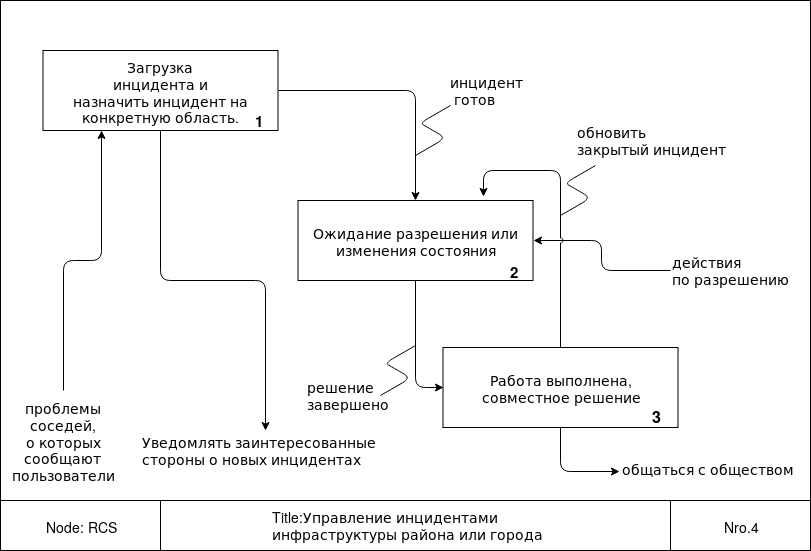
\includegraphics[scale=0.55]{diag_incid.png}
  \caption{Структура системы рекомендаций}
  \label{image:scheme13}
\end{figure}

\begin{table}[]
\centering
\begin{tabular}{|p{4cm}|p{10cm}|}
\hline
\multicolumn{2}{|p{14cm}|}{Область запроса и отдельные подразделы} \\ \hline
Проблемы и улучшения в парках для детей.
& Ремонт.
Увеличения.
Изменения.    \\ \hline
Совершенствование парков и лесов.
& Очистка.
Заказ области.
Безопасность.   \\ \hline
Проблемы в пешеходных зонах.
&  Очистка.
Ремонт тротуаров.
Свет и безопасность.   \\ \hline
Организация дорожного движения.
& Предложения по улучшению трафика.
Заявка на снятие транспортного средства   \\ \hline

\end{tabular}
\centering
\caption{Запрос области.}
\centering
\label{tabla:sencilla3}
\end{table}